\documentclass[11pt]{amsart}

\usepackage[T1]{fontenc}
\usepackage{amsmath,amssymb,amscd,mathtools,mathrsfs}
\usepackage{tikz}
\usepackage{hyperref}
\usepackage[margin=1.15in]{geometry}

\newtheorem{theorem}{Theorem}[section]
\newtheorem{lemma}[theorem]{Lemma}
\newtheorem{proposition}[theorem]{Proposition}
\newtheorem{corollary}[theorem]{Corollary}
\theoremstyle{remark}
\newtheorem{remark}[theorem]{Remark}

\newcommand{\kk}{\mathbb{K}}
\newcommand{\UU}{\mathcal U_q}
\newcommand{\OO}{\mathcal O_q(\mathrm{SL}_n)}
\newcommand{\Sk}{\mathscr S_n}
\newcommand{\rSk}{\overline{\mathscr S}_n}
\newcommand{\Bstar}{\mathfrak B^{*}}
\newcommand{\bplus}{\mathfrak b_+}
\newcommand{\bminus}{\mathfrak b_-}
\newcommand{\slie}{\mathfrak{sl}_n}
\newcommand{\ind}{\mathbf 1}
\DeclareMathOperator{\Span}{span}
\DeclareMathOperator{\id}{id}

\title{Problem 3 -- GPT-6 Astra}
\date{}

\begin{document}
\maketitle

\begin{abstract}
We give an explicit identification of the reduced stated
$\mathrm{SL}_n$-skein algebra of the once-punctured bigon with the
generalized quantum double of the two simply-connected quantum
Borel algebras.  The identification is specified on every horizontal
matrix-coefficient arc.  Its injectivity follows from an ordered
two-arc factorization of the skein algebra, rather than from a
comparison of defining relations alone.  The prescribed diagonal
quotient then identifies the two Cartan tori and gives the
simply-connected quantized enveloping algebra.
\end{abstract}

\section{Coefficients and conventions}

Fix $n\geq 2$.  We give the proof over
\[
  \kk=\mathbb Q(v),\qquad q=v^{2n},\qquad
  \lambda=q-q^{-1}.
\]
Thus all fractional powers needed in the stated skein relations are
available, and $\lambda$ is invertible.  The same argument applies
at non-root-of-unity specializations over a common ground field
containing the required fractional powers.  Throughout,
$\UU(\slie)$ means the unrestricted, simply-connected quantum group,
not a small quantum group.

We use the stated skein conventions of L\^e--Sikora
\cite{LS}: the product $xy$ places $x$ above $y$.
The reduced algebra is the quotient by the bad corner arcs, as in
\cite[Section~7.1]{LY}.

The surface $\Bstar$ is a disk with its top and bottom boundary
points and one interior point removed.  We fix the following
labeling of the horizontal arcs.  Both arcs point to the right;
the first index is the left state and the second is the right state.

\begin{figure}[ht]
\centering
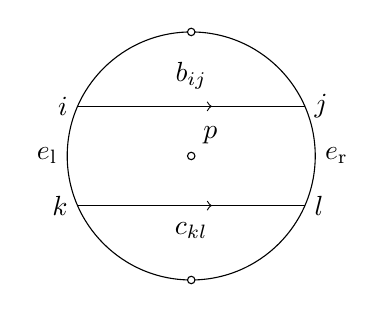
\begin{tikzpicture}[scale=1.05]
  \draw (0,0) circle (1.5);
  \filldraw[fill=white] (0,1.5) circle (.045);
  \filldraw[fill=white] (0,-1.5) circle (.045);
  \filldraw[fill=white] (0,0) circle (.045);
  \node[above right] at (.03,.03) {$p$};

  \draw (-1.375,.6)--(1.375,.6);
  \draw[->] (-.25,.6)--(.25,.6);
  \node[above] at (0,.69) {$b_{ij}$};
  \node[left] at (-1.375,.6) {$i$};
  \node[right] at (1.375,.6) {$j$};

  \draw (-1.375,-.6)--(1.375,-.6);
  \draw[->] (-.25,-.6)--(.25,-.6);
  \node[below] at (0,-.69) {$c_{kl}$};
  \node[left] at (-1.375,-.6) {$k$};
  \node[right] at (1.375,-.6) {$l$};

  \node[left] at (-1.5,0) {$e_{\mathrm l}$};
  \node[right] at (1.5,0) {$e_{\mathrm r}$};
\end{tikzpicture}
\caption{The labeling used in the formulas below.}
\label{fig:bigon}
\end{figure}

At the upper corner the bad right-directed arcs are $b_{ij}$ with
$i<j$.  At the lower corner they are $c_{ij}$ with $i>j$.
Consequently,
\begin{equation}\label{eq:triangular}
 b_{ij}=0\quad(i<j),\qquad
 c_{ij}=0\quad(i>j)
 \qquad\text{in }\rSk(\Bstar).
\end{equation}
The reversal of the inequality at the lower corner is due to the
$180^\circ$ rotation identifying that corner with the standard
upper-corner picture.  If the two letters in a different drawing
are interchanged, the formulas below are to be read with that
interchange.

For the quantum group, put
\[
 \omega_{ai}=\delta_{a,i}-\delta_{a,i+1},
 \qquad
 K_i=\widehat K_i\widehat K_{i+1}^{-1}.
\]
The simply-connected presentation uses
\[
 \widehat K_a^{\pm1}\quad(1\leq a\leq n),
 \qquad E_i,F_i\quad(1\leq i<n),
\]
with commuting toral generators and
\begin{align}
 &\prod_{a=1}^n\widehat K_a=1,
 \label{eq:torus-product}\\
 &\widehat K_a E_i\widehat K_a^{-1}=q^{\omega_{ai}}E_i,
 \qquad
 \widehat K_a F_i\widehat K_a^{-1}=q^{-\omega_{ai}}F_i,
 \label{eq:torus-weights}\\
 &[E_i,F_j]=\delta_{ij}\frac{K_i-K_i^{-1}}{\lambda}.
 \label{eq:DJ-comm}
\end{align}
For $X=E$ and $X=F$ the remaining relations are
\begin{align}
 X_iX_j&=X_jX_i &&(|i-j|>1),\label{eq:far}\\
 X_i^2X_j-(q+q^{-1})X_iX_jX_i+X_jX_i^2&=0
 &&(|i-j|=1).\label{eq:Serre}
\end{align}
Our coproduct convention is
\begin{equation}\label{eq:coproduct}
 \begin{split}
 \Delta(\widehat K_a)&=\widehat K_a\otimes\widehat K_a,\\
 \Delta(E_i)&=E_i\otimes K_i+1\otimes E_i,\\
 \Delta(F_i)&=F_i\otimes1+K_i^{-1}\otimes F_i.
 \end{split}
\end{equation}
These conventions specify the extended quantum group in the
question; see \cite{KS}.  The corresponding Borel presentations
use the toral relations and the respective $E$- or $F$-relations.
They also follow from the quantum-matrix realizations recalled in
Lemma~\ref{lem:borel} below.

\section{The skein-theoretic matrix calculation}

Let $V=\kk^n$, let $e_{ab}$ denote its matrix units, and set
\begin{equation}\label{eq:R}
 R=q^{-1/n}\left(
       \sum_{a,b=1}^n q^{\delta_{ab}}e_{aa}\otimes e_{bb}
       +\lambda\sum_{a>b}e_{ab}\otimes e_{ba}
     \right).
\end{equation}
The braiding matrix is $PR$, where $P$ interchanges the tensor
factors.  This is the normalization used in
\cite[Equation~(9)]{LS}.

For a matrix $T=(t_{ij})$, write
$T_1=T\otimes I_n$ and $T_2=I_n\otimes T$.
The standard quantum coordinate algebra $\OO$ has presentation
\begin{equation}\label{eq:FRT}
 RT_1T_2=T_2T_1R,\qquad
 \det\nolimits_q(T)=1,
\end{equation}
where
\[
 \det\nolimits_q(T)
   =\sum_{\sigma\in S_n}(-q)^{\ell(\sigma)}
       t_{1,\sigma(1)}\cdots t_{n,\sigma(n)}.
\]
Define its triangular quotients
\begin{equation}\label{eq:triangular-algebras}
 \mathcal T^-=\OO/(t_{ij}:i<j),
 \qquad
 \mathcal T^+=\OO/(t_{ij}:i>j).
\end{equation}

\begin{lemma}[Two-arc matrix calculation]\label{lem:skein}
Let $A=\rSk(\Bstar)$, and let
$B=(b_{ij})$ and $C=(c_{ij})$ be as in
Figure~\ref{fig:bigon}.
\begin{enumerate}
\item
$B$ and $C$ satisfy \eqref{eq:FRT}.  Moreover, $B$ is lower
triangular and $C$ is upper triangular.
\item
The mixed relation is
\begin{equation}\label{eq:mixed-matrix}
 RB_1C_2=C_2B_1R.
\end{equation}
Equivalently, for all $i,j,k,l$,
\begin{equation}\label{eq:mixed-components}
 \begin{split}
 q^{\delta_{ik}}b_{ij}c_{kl}
 -q^{\delta_{jl}}c_{kl}b_{ij}
 =\lambda\bigl(
       \ind_{j<l}c_{kj}b_{il}
       -\ind_{k<i}b_{kj}c_{il}
     \bigr).
 \end{split}
\end{equation}
\item
The homomorphisms from $\mathcal T^-$ and $\mathcal T^+$ determined
by $T\mapsto B$ and $T\mapsto C$ are injective, and multiplication
induces a vector-space isomorphism
\begin{equation}\label{eq:skein-factorization}
 \mathcal T^-\otimes_\kk\mathcal T^+
       \xrightarrow{\ \sim\ } A,\qquad
 f\otimes g\longmapsto f(B)g(C).
\end{equation}
This is a vector-space assertion, not an assertion that the
ordinary tensor-product multiplication is preserved.
\end{enumerate}
\end{lemma}

\begin{proof}
A thin neighborhood of either horizontal arc is an ideal bigon.
The bigon theorem \cite[Theorem~6.3]{LS} identifies its stated skein
algebra with $\OO$, with the right-directed stated arcs as the
matrix generators.  This proves the quantum-matrix and determinant
relations.  Equation~\eqref{eq:triangular} gives the asserted
triangularity.

% Online source for the bigon theorem and its matrix-coefficient normalization: ([arxiv.org](https://arxiv.org/pdf/2201.00045))

Here are the boundary-exchange details for the mixed relation.
They hold already in the unreduced algebra.  Consider the two
disjoint arcs with $c$ higher than $b$ at the left boundary and $b$
higher than $c$ at the right boundary.  Denote the resulting
mixed-height diagram, with external state pairs $(i,k)$ and
$(j,l)$, by $W_{ik;jl}$.  Applying the boundary height-exchange
relation at the left or at the right gives, respectively,
\begin{equation}\label{eq:two-exchanges}
 W_{ik;jl}
   =\sum_{a,b}R_{ik,ab}\,b_{aj}c_{bl}
   =\sum_{a,b}c_{kb}b_{ia}\,R_{ab,jl}.
\end{equation}
Here the flip in the braiding $PR$ has been removed by recording
the indices in the order of the two arcs.  Thus the coefficients
appearing in the two exchanges are
\[
 \begin{split}
 R_{ik,ab}
 &=q^{-1/n}\left(
      q^{\delta_{ik}}\delta_{ia}\delta_{kb}
      +\lambda\ind_{k<i}\delta_{ka}\delta_{ib}
   \right),\\
 R_{ab,jl}
 &=q^{-1/n}\left(
      q^{\delta_{jl}}\delta_{aj}\delta_{bl}
      +\lambda\ind_{j<l}\delta_{al}\delta_{bj}
   \right).
 \end{split}
\]
These are precisely the boundary braiding coefficients
\eqref{eq:R}; the boundary relations and their braiding
interpretation are those of \cite[Section~4 and Theorem~6.4]{LS}.
Substitution into \eqref{eq:two-exchanges}, followed by cancellation
of $q^{-1/n}$, proves \eqref{eq:mixed-components}.

% Online source for the braiding matrix used in the boundary-exchange calculation: ([arxiv.org](https://arxiv.org/pdf/2201.00045))

It remains to prove the vector-space assertion, including the
absence of additional relations after reduction.
Write $S=\Sk(\Bstar)$ for the unreduced algebra, and temporarily
use $b,c$ for the unreduced arcs.  They form the standard saturated
two-arc system for $\Bstar$: together with the boundary edges they
give a groupoid spine of the punctured bigon.  The ordered-arc
factorization theorem, with the $b$-neighborhood above the
$c$-neighborhood at both boundary edges, gives
\begin{equation}\label{eq:unreduced-factorization}
 m:\OO\otimes_\kk\OO\xrightarrow{\ \sim\ }S,\qquad
 f\otimes g\longmapsto f(B)g(C).
\end{equation}
The relevant result permits arbitrary orders at the boundary
edges; see \cite[Corollary~8.14]{LS}.

% Online source for the arbitrary-boundary-order factorization theorem: ([arxiv.org](https://arxiv.org/pdf/2201.00045))

Let $J_b$ be the ideal of the first copy of $\OO$ generated by
$t_{ij}$ with $i<j$, and let $J_c$ be the ideal of the second copy
generated by $t_{ij}$ with $i>j$.
Let $I_{\mathrm{top}}$ and $I_{\mathrm{bottom}}$ be the respective
bad-corner ideals in $S$.

The bad-arc normality theorem
\cite[Theorem~7.2, especially Equation~(128)]{LY} says that each
corner ideal is both the left and the right ideal generated by
either one of its two oriented families of bad arcs.  In our
notation this gives
\[
 I_{\mathrm{top}}
   =\Span_\kk\{b_{ij}:i<j\}\,S,
 \qquad
 I_{\mathrm{bottom}}
   =S\,\Span_\kk\{c_{ij}:i>j\}.
\]
In particular, reversed orientations introduce no further ideal.

% Online source for the bad-arc normality theorem, including the equivalence of the two orientations: ([arxiv.org](https://arxiv.org/pdf/2303.08082))

Using \eqref{eq:unreduced-factorization}, the first equality implies
\[
 I_{\mathrm{top}}\subseteq m(J_b\otimes\OO).
\]
The reverse inclusion holds because $I_{\mathrm{top}}$ is a
two-sided ideal containing the generators of $J_b$.  Hence
\[
 I_{\mathrm{top}}=m(J_b\otimes\OO).
\]
The same argument, using the displayed right-ideal description at
the lower corner, gives
\[
 I_{\mathrm{bottom}}=m(\OO\otimes J_c).
\]
Therefore
\[
 I^{\mathrm{bad}}
   =m\bigl(J_b\otimes\OO+\OO\otimes J_c\bigr).
\]
Taking the quotient of the vector-space isomorphism
\eqref{eq:unreduced-factorization} proves
\eqref{eq:skein-factorization}.  The injectivity of the two factor
maps follows as well.
\end{proof}

We record two elementary consequences that will also make the
eventual isomorphism explicit on all the arcs.  The diagonal
entries of either triangular quantum matrix commute, and
\begin{equation}\label{eq:diagonal-units}
 \prod_{a=1}^n b_{aa}=\prod_{a=1}^n c_{aa}=1.
\end{equation}
Thus every diagonal entry is invertible.  Expanding the
quantum-matrix relation on the indicated $2\times2$ submatrices
gives, for $i<j-1$,
\begin{align}
 b_{ji}
 &=\lambda^{-1}b_{j-1,j-1}^{-1}
     [b_{j-1,i},b_{j,j-1}],
 \label{eq:lower-recursion}\\
 c_{ij}
 &=\lambda^{-1}c_{j-1,j-1}^{-1}
     [c_{i,j-1},c_{j-1,j}].
 \label{eq:upper-recursion}
\end{align}
Indeed, these are the relations $ad-da=\lambda bc$ for rows
$j-1,j$ and columns $i,j-1$, and for rows $i,j-1$ and columns
$j-1,j$, respectively.  In each case the diagonal factor on the
right commutes with the opposite off-diagonal factor.
Consequently, each triangular algebra is generated by its diagonal
and immediately adjacent off-diagonal entries.

\section{The quantum Borel algebras and their double}

\subsection{Triangular matrix realizations}

Write
\[
 H_-=\UU(\bminus),\qquad H_+=\UU(\bplus).
\]

\begin{lemma}[Borel matrix realizations]\label{lem:borel}
There are algebra isomorphisms
\[
 \eta_-:H_-\xrightarrow{\ \sim\ }\mathcal T^-,
 \qquad
 \eta_+:H_+\xrightarrow{\ \sim\ }\mathcal T^+
\]
given by
\begin{align}
 \eta_-(\widehat K_a)&=b_{aa}^{-1},
 &
 \eta_-(F_i)&=\lambda^{-1}b_{i+1,i+1}^{-1}b_{i+1,i},
 \label{eq:eta-minus}\\
 \eta_+(\widehat K_a)&=c_{aa},
 &
 \eta_+(E_i)&=-\lambda^{-1}c_{i,i+1}c_{i+1,i+1}^{-1}.
 \label{eq:eta-plus}
\end{align}
\end{lemma}

\begin{proof}
For $\mathfrak{gl}_n$, with independent toral generators
$G_1,\ldots,G_n$, these are exactly the algebra isomorphisms
$\zeta_-$ and $\zeta_+$ in \cite[Section~2.4]{Gav}.
Their inverses on adjacent entries are
\[
 t_{i+1,i}\longmapsto\lambda G_{i+1}^{-1}F_i,
 \qquad
 t_{i,i+1}\longmapsto-\lambda E_iG_{i+1},
\]
and the diagonal entries map to $G_a^{-1}$ and $G_a$,
respectively.

Impose the central relation $\prod_aG_a=1$.
On the matrix sides its image is the relation that the product
of the diagonal entries is $1$.  For a triangular matrix this is
exactly the quantum determinant-one relation.  Taking these
quotients gives \eqref{eq:eta-minus}--\eqref{eq:eta-plus}.
The toral lattice is
$\mathbb Z^n/\mathbb Z(1,\ldots,1)$, namely the weight lattice of
type $A_{n-1}$, so the resulting Borel algebras are the
simply-connected ones.

Only the algebra assertion of \cite[Section~2.4]{Gav} is used:
the coproduct convention there is opposite to
\eqref{eq:coproduct}.
\end{proof}

% Online source containing the explicit Borel isomorphisms and their inverses: ([arxiv.org](https://arxiv.org/pdf/math/0403346))

\subsection{A presentation of the generalized double}

Let
\[
 D=H_-\bowtie H_+
\]
be the generalized quantum double for the pairing in the question.
We denote its two toral copies by $\widehat K_a^-$ and
$\widehat K_a^+$, and set
\[
 K_i^-=\widehat K_i^-(\widehat K_{i+1}^-)^{-1},
 \qquad
 K_i^+=\widehat K_i^+(\widehat K_{i+1}^+)^{-1}.
\]
The superscript $-$ labels the negative Borel copy; it does not
mean an inverse.

For clarity, we specify the double convention.  The skew pairing
$\tau:H_+\otimes H_-\to\kk$ satisfies
\[
 \begin{split}
 \tau(xx',y)&=\tau(x,y_{(1)})\tau(x',y_{(2)}),\\
 \tau(x,yy')&=\tau(x_{(1)},y')\tau(x_{(2)},y),
 \end{split}
\]
and has generator values
\begin{equation}\label{eq:pairing}
 \begin{split}
 \tau(\widehat K_a,\widehat K_b)&=q^{1/n-\delta_{ab}},\\
 \tau(E_i,F_j)&=-\delta_{ij}\lambda^{-1},\\
 \tau(\widehat K_a,F_j)&=\tau(E_i,\widehat K_b)=0.
 \end{split}
\end{equation}
The underlying vector space of $D$ is $H_-\otimes H_+$, with
multiplication identifying each factor with a subalgebra.  Its
exchange convention is
\begin{equation}\label{eq:double-exchange}
 \sum\tau(x_{(1)},y_{(1)})x_{(2)}y_{(2)}
 =
 \sum y_{(1)}x_{(1)}\tau(x_{(2)},y_{(2)}),
 \qquad x\in H_+,\quad y\in H_-.
\end{equation}
Writing this convention explicitly avoids ambiguity with
opposite-double conventions.

\begin{lemma}[Presentation of the double]\label{lem:double}
The algebra $D$ is presented by the two Borel presentations and
the following mixed relations:
\begin{align}
 [\widehat K_a^+,\widehat K_b^-]&=0,
 \label{eq:double-tori}\\
 \widehat K_a^+F_i(\widehat K_a^+)^{-1}
   &=q^{-\omega_{ai}}F_i,
 &
 \widehat K_a^-E_i(\widehat K_a^-)^{-1}
   &=q^{\omega_{ai}}E_i,
 \label{eq:double-weights}\\
 [E_i,F_j]
   &=\delta_{ij}\frac{K_i^+-(K_i^-)^{-1}}{\lambda}.
 \label{eq:double-EF}
\end{align}
\end{lemma}

\begin{proof}
First derive the relations in $D$.
For the toral terms,
\[
 \tau(\widehat K_a,K_i)
  =\frac{q^{1/n-\delta_{ai}}}
         {q^{1/n-\delta_{a,i+1}}}
  =q^{-\omega_{ai}}.
\]
Substitution into \eqref{eq:double-exchange} proves
\eqref{eq:double-tori} and \eqref{eq:double-weights}.

For $x=E_i$ and $y=F_j$, the left and right sides of
\eqref{eq:double-exchange}, using \eqref{eq:coproduct}, are
\[
 E_iF_j-\delta_{ij}\lambda^{-1}K_i^+,
 \qquad
 F_jE_i-\delta_{ij}\lambda^{-1}(K_j^-)^{-1},
\]
respectively.  This proves \eqref{eq:double-EF}.

To see that these are a complete set of mixed relations, let
$D_0$ be the algebra given by the two Borel presentations and
\eqref{eq:double-tori}--\eqref{eq:double-EF}.  The derived relations
give a surjection $D_0\to D$.

They also allow every word in $D_0$ to be written as a sum of
words with the negative Borel generators first and the positive
Borel generators second.  Indeed, the toral exchanges merely
introduce scalars; the exchange of $E_i$ with $F_j$ has a reordered
term and terms with fewer $E$'s and $F$'s.  Induction first on the
number of such generators and then on the number of mixed
inversions proves the assertion.  Hence multiplication gives a
surjection
\[
 H_-\otimes H_+\longrightarrow D_0.
\]
Its composition with $D_0\to D$ is the defining vector-space
isomorphism $H_-\otimes H_+\to D$.  It follows that both maps are
isomorphisms, proving the presentation.
\end{proof}

\section{The explicit isomorphism}

Define elements of the two Borel factors, for $1\leq i<j\leq n$,
by
\begin{align}
 \mathsf F_{i,i+1}&=F_i,
 &
 \mathsf F_{ij}
   &=\mathsf F_{i,j-1}F_{j-1}
       -q^{-1}F_{j-1}\mathsf F_{i,j-1}
       &&(j>i+1),
 \label{eq:F-roots}\\
 \mathsf E_{i,i+1}&=E_i,
 &
 \mathsf E_{ij}
   &=E_{j-1}\mathsf E_{i,j-1}
       -q\,\mathsf E_{i,j-1}E_{j-1}
       &&(j>i+1).
 \label{eq:E-roots}
\end{align}
These recursions fix all root-vector normalizations needed below.

\begin{theorem}\label{thm:main}
There is an algebra isomorphism
\[
 \Phi:\rSk(\Bstar)\xrightarrow{\ \sim\ }
       \UU(\bminus)\bowtie\UU(\bplus)
\]
given on the horizontal arcs by
\begin{align}
 \Phi(b_{aa})&=(\widehat K_a^-)^{-1},
 &
 \Phi(c_{aa})&=\widehat K_a^+,
 \label{eq:Phi-diagonal}\\
 \Phi(b_{ji})&=\lambda(\widehat K_j^-)^{-1}\mathsf F_{ij},
 &
 \Phi(c_{ij})&=-\lambda\mathsf E_{ij}\widehat K_j^+
       &&(i<j).
 \label{eq:Phi-offdiagonal}
\end{align}
The other off-diagonal arcs vanish by
\eqref{eq:triangular}.

Equivalently, the inverse isomorphism $\Psi=\Phi^{-1}$ is
determined by
\begin{align}
 \Psi(\widehat K_a^-)&=b_{aa}^{-1},
 &
 \Psi(\widehat K_a^+)&=c_{aa},
 \label{eq:Psi-tori}\\
 \Psi(F_i)&=\lambda^{-1}b_{i+1,i+1}^{-1}b_{i+1,i},
 &
 \Psi(E_i)&=-\lambda^{-1}c_{i,i+1}c_{i+1,i+1}^{-1}.
 \label{eq:Psi-EF}
\end{align}
\end{theorem}

\begin{proof}
We first construct $\Psi$ and prove that it is an isomorphism.

For brevity put, in $A=\rSk(\Bstar)$,
\[
 d_a=b_{aa},\qquad t_a=c_{aa},\qquad
 x_i=b_{i+1,i},\qquad y_i=c_{i,i+1}.
\]
The diagonal elements are invertible by
\eqref{eq:diagonal-units}.  Lemma~\ref{lem:borel} gives algebra
homomorphisms from the two Borel factors to $A$ with the values
\eqref{eq:Psi-tori}--\eqref{eq:Psi-EF}.  Thus it remains to check the
mixed relations in Lemma~\ref{lem:double}.

The internal quantum-matrix relations and
\eqref{eq:mixed-components} give
\begin{equation}\label{eq:diagonal-commute}
 [d_a,d_b]=[t_a,t_b]=[d_a,t_b]=0
\end{equation}
and
\begin{equation}\label{eq:entry-weights}
 \begin{array}{ll}
 d_ax_i=q^{\omega_{ai}}x_id_a,
   & t_ax_i=q^{-\omega_{ai}}x_it_a,\\[2pt]
 d_ay_i=q^{-\omega_{ai}}y_id_a,
   & t_ay_i=q^{\omega_{ai}}y_it_a.
 \end{array}
\end{equation}
For example, setting the first matrix entry in
\eqref{eq:mixed-components} equal to $b_{aa}$ makes both correction
terms vanish by lower triangularity, and yields
\[
 d_ac_{kl}=q^{\delta_{al}-\delta_{ak}}c_{kl}d_a.
\]
Setting the second entry equal to $c_{aa}$ gives
\[
 t_ab_{kl}=q^{\delta_{ak}-\delta_{al}}b_{kl}t_a.
\]
These are the mixed assertions in \eqref{eq:entry-weights}; the
internal ones are obtained in the same way from the single-matrix
relation.

Write
\[
 \mathcal F_i=\lambda^{-1}d_{i+1}^{-1}x_i,
 \qquad
 \mathcal E_i=-\lambda^{-1}y_it_{i+1}^{-1}.
\]
Equations~\eqref{eq:diagonal-commute} and
\eqref{eq:entry-weights} immediately give
\[
 t_a\mathcal F_it_a^{-1}=q^{-\omega_{ai}}\mathcal F_i,
 \qquad
 d_a^{-1}\mathcal E_id_a=q^{\omega_{ai}}\mathcal E_i.
\]
Thus the mixed toral relations are satisfied.

For the remaining mixed relation, substitute
\[
 (i,k;j,l)=(j+1,i;j,i+1)
\]
into \eqref{eq:mixed-components}.  Triangularity makes both
correction terms vanish unless $i=j$, so that
\begin{equation}\label{eq:simple-mixed}
 q^{\delta_{i,j+1}}x_jy_i
 -q^{\delta_{j,i+1}}y_ix_j
 =\lambda\delta_{ij}(d_{i+1}t_i-d_it_{i+1}).
\end{equation}
Using \eqref{eq:entry-weights} to move the diagonal factors gives
\begin{align}
 [\mathcal E_i,\mathcal F_j]
 &=
 \lambda^{-2}d_{j+1}^{-1}
 \left(
   x_jy_i
   -q^{\delta_{j,i+1}-\delta_{i,j+1}}y_ix_j
 \right)t_{i+1}^{-1}
 \notag\\
 &=
 \delta_{ij}\lambda^{-1}
       d_{i+1}^{-1}(d_{i+1}t_i-d_it_{i+1})t_{i+1}^{-1}
 \notag\\
 &=\delta_{ij}\frac{
          t_it_{i+1}^{-1}-d_id_{i+1}^{-1}
        }{\lambda}.
 \label{eq:computed-commutator}
\end{align}
But under the proposed map,
\[
 K_i^+\longmapsto t_it_{i+1}^{-1},
 \qquad
 (K_i^-)^{-1}\longmapsto d_id_{i+1}^{-1}.
\]
Therefore \eqref{eq:computed-commutator} is precisely
\eqref{eq:double-EF}.  Lemma~\ref{lem:double} now supplies an
algebra homomorphism
\[
 \Psi:D\longrightarrow A
\]
with the required values.

We prove its bijectivity without making an unsupported
presentation claim about $A$.  The following diagram commutes:
\[
\begin{CD}
 H_-\otimes_\kk H_+ @>{m_D}>> D\\
 @V{\eta_-\otimes\eta_+}V{\cong}V @VV{\Psi}V\\
 \mathcal T^-\otimes_\kk\mathcal T^+
       @>{m_A}>> A .
\end{CD}
\]
The top arrow is the defining vector-space isomorphism for the
generalized double.  The left arrow is an isomorphism by
Lemma~\ref{lem:borel}, and the bottom arrow is an isomorphism by
Lemma~\ref{lem:skein}.  Consequently $\Psi$ is a vector-space
isomorphism and hence an algebra isomorphism.

It remains to verify the formulas for its inverse on the
non-adjacent entries.  The inverse formulas on the diagonal and
adjacent entries follow directly from
\eqref{eq:Psi-tori}--\eqref{eq:Psi-EF}.  For completeness, the
induction using \eqref{eq:lower-recursion} and
\eqref{eq:upper-recursion} is as follows.

Put
\[
 m_a=(\widehat K_a^-)^{-1},
 \qquad p_a=\widehat K_a^+.
\]
For $i<j-1$, assume the asserted formulas at distance $j-i-1$.
The toral weight relations give
\[
 \begin{split}
 &\lambda^{-1}m_{j-1}^{-1}
   [\,\lambda m_{j-1}\mathsf F_{i,j-1},
      \lambda m_jF_{j-1}\,]\\
 &\hspace{25mm}
 =\lambda m_j
    \bigl(\mathsf F_{i,j-1}F_{j-1}
            -q^{-1}F_{j-1}\mathsf F_{i,j-1}\bigr)
 =\lambda m_j\mathsf F_{ij}.
 \end{split}
\]
Here $m_j$ commutes with $\mathsf F_{i,j-1}$ and
$F_{j-1}m_{j-1}=q^{-1}m_{j-1}F_{j-1}$.
This proves the lower-triangular formula.

Similarly,
\[
 \begin{split}
 &\lambda^{-1}p_{j-1}^{-1}
   [\,-\lambda\mathsf E_{i,j-1}p_{j-1},
      -\lambda E_{j-1}p_j\,]\\
 &\hspace{25mm}
 =-\lambda
   \bigl(E_{j-1}\mathsf E_{i,j-1}
            -q\mathsf E_{i,j-1}E_{j-1}\bigr)p_j
 =-\lambda\mathsf E_{ij}p_j.
 \end{split}
\]
Indeed, $p_j$ commutes with $\mathsf E_{i,j-1}$,
$p_{j-1}E_{j-1}=qE_{j-1}p_{j-1}$, and the total weight of
$\mathsf E_{i,j-1}E_{j-1}$ has zero coefficient at $j-1$.
The latter weight statement follows by induction directly from
\eqref{eq:E-roots}.  This proves the upper-triangular formula and
completes the proof.
\end{proof}

\section{The diagonal quotient}

\begin{theorem}\label{thm:quotient}
Let $I$ be the two-sided ideal of $\rSk(\Bstar)$ generated by
\[
 b_{aa}c_{aa}-1,\qquad 1\leq a\leq n.
\]
Then
\[
 \rSk(\Bstar)/I\cong\UU(\slie),
\]
where the quantum group is the simply-connected one.

Writing bars for classes in the quotient, the inverse
isomorphism from $\UU(\slie)$ is explicitly
\begin{align}
 \widehat K_a
   &\longmapsto \overline c_{aa}
      =\overline b_{aa}^{\, -1},
 \label{eq:quotient-torus}\\
 E_i
   &\longmapsto
       -\lambda^{-1}\overline c_{i,i+1}
                         \overline c_{i+1,i+1}^{\, -1},
 \label{eq:quotient-E}\\
 F_i
   &\longmapsto
       \lambda^{-1}\overline b_{i+1,i+1}^{\, -1}
                        \overline b_{i+1,i}.
 \label{eq:quotient-F}
\end{align}
\end{theorem}

\begin{proof}
By Theorem~\ref{thm:main},
\[
 \Phi(b_{aa}c_{aa}-1)
   =(\widehat K_a^-)^{-1}\widehat K_a^+-1.
\]
Since $\widehat K_a^-$ is a unit, these elements generate the
same ideal of $D$ as
\[
 \widehat K_a^+-\widehat K_a^-,
 \qquad 1\leq a\leq n.
\]
Denote that ideal by $J$.  Hence $\Phi(I)=J$ and
\begin{equation}\label{eq:quotient-double}
 \rSk(\Bstar)/I\cong D/J.
\end{equation}

There is a surjective homomorphism
\[
 \pi:D\longrightarrow\UU(\slie)
\]
sending both $\widehat K_a^-$ and $\widehat K_a^+$ to
$\widehat K_a$ and sending $E_i,F_i$ to the identically named
generators.  To check it, use Lemma~\ref{lem:double}:
the only new commutator becomes
\[
 [E_i,F_j]
   =\delta_{ij}\frac{K_i-K_i^{-1}}{\lambda},
\]
and all the other relations become
\eqref{eq:torus-product}--\eqref{eq:Serre}.
Clearly $J\subseteq\ker\pi$.

Conversely, in $D/J$ the two toral copies agree.  Their common
images together with the images of $E_i,F_i$ satisfy the entire
presentation \eqref{eq:torus-product}--\eqref{eq:Serre}.  They
therefore define a homomorphism
\[
 \UU(\slie)\longrightarrow D/J.
\]
This homomorphism and the map induced by $\pi$ are inverse on
every generator.  Consequently
\[
 D/J\cong\UU(\slie)
 \qquad\text{and}\qquad \ker\pi=J.
\]
Together with \eqref{eq:quotient-double}, this proves the claimed
quotient, including the assertion that no further relations have
been introduced.  Formulas
\eqref{eq:quotient-torus}--\eqref{eq:quotient-F} are the
specializations of \eqref{eq:Psi-tori}--\eqref{eq:Psi-EF}.
\end{proof}

\begin{remark}
The elements $b_{aa}c_{aa}$ are central.  Under $\Phi$ they become
$(\widehat K_a^-)^{-1}\widehat K_a^+$, and the two toral copies
have identical conjugation actions on every $E_i$ and $F_i$.
Furthermore,
\[
 \prod_{a=1}^n b_{aa}c_{aa}=1.
\]
Thus the quotient identifies the two full weight-lattice tori;
there are only $n-1$ independent diagonal identifications.
This is also why the conclusion is the simply-connected quantum
group rather than its root-lattice form.
\end{remark}

\begin{remark}[Parameter qualification]
The factors $\lambda^{-1}$ are essential to the identification
with the usual Chevalley generators.  At $q=\pm1$ the skew pairing
displayed in the question itself is undefined.  Statements at
such parameters require an integral-form reformulation and are
not obtained by substituting into the formulas above.
\end{remark}

\begin{thebibliography}{99}

\bibitem{Gav}
F.~Gavarini,
\emph{Presentation by Borel subalgebras and Chevalley generators
for quantum enveloping algebras},
Proc. Edinburgh Math. Soc. (2) \textbf{49} (2006), no.~2,
291--308.
See also arXiv:math/0403346v3; the section numbering cited above
is that of this version.

\bibitem{KS}
A.~Klimyk and K.~Schm\"udgen,
\emph{Quantum Groups and Their Representations},
Texts and Monographs in Physics,
Springer-Verlag, Berlin, 1997.

\bibitem{LS}
T.~T.~Q.~L\^e and A.~S.~Sikora,
\emph{Stated $\mathrm{SL}(n)$-skein modules and algebras},
J. Topol. \textbf{17} (2024), no.~3, e12350.
See also arXiv:2201.00045; the theorem and corollary numbering
cited above refers to the 85-page arXiv text.

\bibitem{LY}
T.~T.~Q.~L\^e and T.~Yu,
\emph{Quantum traces for $\mathrm{SL}_n$-skein algebras},
arXiv:2303.08082v2, May 28, 2025.

\end{thebibliography}
\end{document}